
\chapter{Macro-programming}\label{chap:macro-programming}%\mtcaddchapter
\minitoc% Creating an actual minitoc
\newcommand{\q}[1]{\texttt{#1}}
%% TODO REMEMBER TO DISCUSS THE GRADIENT
Macroprogramming, as a paradigm, 
 has emerged as a pivotal approach in the realm of distributed systems. 
%
It offers a unique perspective, 
 allowing developers to express the \emph{macroscopic behaviour} of a collective system using a singular program.
% 
This chapter delves into the intricacies of macroprogramming, 
 its historical evolution, and its significance in the modern computational landscape, 
 leading to aggregate computing -- a novel macro-programming approach for 
 programming collective self-organizing behaviours in highly scalable and distributed systems.

\begin{figure}
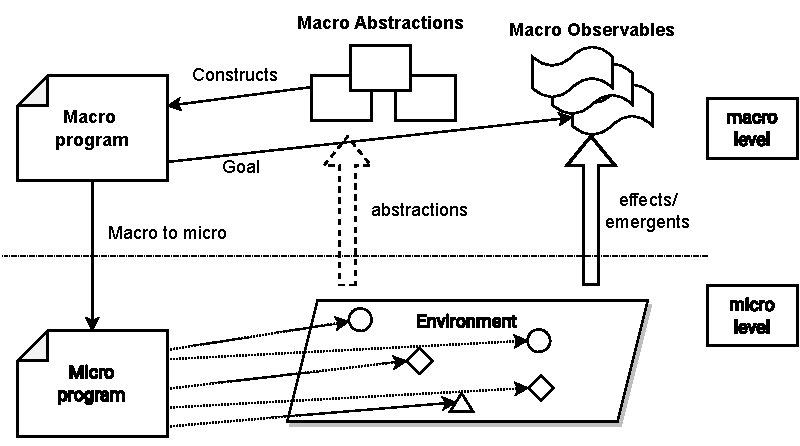
\includegraphics[width=\textwidth]{chapters/img/macroprogramming.drawio}
\caption{Overview of macroprogramming}\label{macro:fig:macro-programming}
\end{figure}
\section{The Essence of Macroprogramming}
Macroprogramming~\cite{casadei2023macroprogramming} emphasizes the overarching behaviour of a system, 
 abstracting the intricacies of individual components. 
 This abstraction is crucial for systems where collective behaviour is the objective of the design process.

The primary motivation behind macroprogramming 
 is to simplify the design and development of complex systems. 
 By providing a higher-level perspective, 
 it allows developers to address system-wide concerns without getting bogged down by the details of individual components. 
 Indeed, developers should focus solely on the system's overall behaviour, rather than worrying about its technological details, individual component capabilities, or communication protocols.
This not only streamlines the development process but also ensures that the system's behaviour is \emph{consistent} and \emph{predictable}.

In essence, macroprogramming is about seeing the \emph{forest} for the \emph{trees}. 
 It recognizes that while individual components (or trees) are essential,
 understanding and managing their collective behaviour (or the forest) is of paramount importance. 
This perspective is particularly relevant in today's interconnected world, 
 where systems often comprise numerous components that need to work in harmony.

Furthermore, macroprogramming leverages macro-level abstractions, 
 such as \emph{collective states}, \emph{groups}, or \emph{spatiotemporal} patterns. 
 These abstractions provide a structured way to think about and design systems, ensuring that they are both \emph{robust} and \emph{adaptable}. 
By focusing on these higher-level abstractions, 
 macroprogramming allows for a more intuitive and efficient approach to system design, 
 making it an indispensable tool in the modern developer's toolkit.
\Cref{macro:fig:macro-programming} provides an overview of the idea behind this paradigm.

Diving deeper into the terminology, 
 terms like ``system programming'', ``centralized programming'', and ``high-level programming'' 
 have been used in various contexts, leading to potential confusion. 
% 
Among these, domain-specific terms like ``global-level programming'', ``swarm programming'', and 
 ``aggregate programming'' stand out. 
%
These terms reflect the diverse perspectives from which macroprogramming can be approached, 
 emphasizing the need for a unified framework that can consolidate these diverse viewpoints. 
%
Such a framework would not only provide clarity but also pave the way for innovative solutions in the realm of systemic behaviour modelling.

\section{Conceptual Framework}

\subsection{Preliminaries}
Macroprogramming addresses the challenge of programming the behaviour of a computational system \( S \), composed of multiple computational entities. 
 Given two entities \( A \) and \( B \) within this system, 
 there are three primary modes to influence their behaviour to promote properties ascribable to \( S \):
\begin{enumerate}
    \item Altering their context, 
    indirectly influencing them. 
    For instance, a change in sensor \( A \) might subsequently affect \( B \).
    \item Interaction, such as triggering their behaviour. 
    If \( A \) is an actuator, its actions might influence \( B \).
    \item Setting their behaviour to produce certain global outcomes when activated.
\end{enumerate}
The term ``program'' refers to an abstract description executable by a computational entity. 
 Modes (1) and (2) allow an external entity \( C \) to influence \( A \) or \( B \), and consequently \( S \).

\subsection{Macroprogramming: Definition and Basic Concepts}
\sloppy
Macroprogramming is defined as an abstract paradigm for programming the macroscopic behaviour of systems of computational entities. 
 As a paradigm, it's an approach rooted in a mathematical theory or a set of coherent principles. 
 The foundational principles of macroprogramming include:
\begin{itemize}
    \item Micro-macro distinction: Recognizing two primary system levels -- macro (global structures) and micro (computational entities).
    \item Macroscopic perspective: Focusing on the system's macroscopic aspects, 
    considering micro-level entities from a global perspective.
    \item Microprogram: The result of macroprogramming, a program executed by the system adopting the macroscopic perspective.
    \item Macro-to-micro mapping: Implementing how a macro program is executed by the system, 
    defining a logic to map macro instructions to micro-level behaviours.
\end{itemize}

\subsubsection{On Micro-Macro and Local-Global Distinction}
The micro-macro distinction is prevalent in various scientific areas, 
 distinguishing smaller elements from larger ones. 
 For programming, a system can be defined based on a boundary condition, 
 distinguishing between the micro and macro dimensions. 
 The goal of macroprogramming is closely tied to the concept of emergence, 
 analysing the relationships between microscopic and macroscopic states.


\subsubsection{On Collectives}
Macroprogramming often targets \emph{collectives}, 
 groups of similar entities sharing common traits or goals. 
% 
While heterogeneous collectives exist, 
 they tend to complicate macroprogramming by emphasizing individual perspectives or widening the macro-to-micro gap.

\subsubsection{On Declaratively}
Declarativity is a hallmark of macroprogramming, 
 focusing on the computation's goal rather than its method. 
 This approach abstracts away specific computational aspects, 
 offering high-level abstractions tailored to specific application domains, 
 often resulting in Domain-Specific Languages (DSLs).

\subsection{Historical Evolution and Context}
The historical roots of macroprogramming can be traced back to the pioneering work of Newton and Welsh~\cite{newton2004region}. 
 Their research laid the foundation for the application of macroprogramming in the domain of Wireless Sensor Networks (WSNs). 
 These networks, characterized by embedded units equipped with processing, communication, and sensing capabilities, presented unique challenges that necessitated a macroscopic view for effective data processing and logic description. 
The emphasis was on capturing the collective behaviour of these sensor nodes, 
 ensuring efficient data aggregation, processing, and communication.

WSNs were among the first systems that required a departure from traditional programming paradigms. 
 Given the distributed nature of these networks and the limited resources of individual sensor nodes, 
 there was a pressing need to optimize both computation and communication. 
 Macroprogramming emerged as a solution, 
 allowing developers to focus on the overall behaviour of the network rather than the intricacies of individual nodes.

As technology evolved, so did the applications of macroprogramming. 
 The rise of the Internet of Things (IoT) in the subsequent years brought forth a plethora of interconnected devices, each with its own set of capabilities and functions. 
 The complexity of these systems further underscored the importance of a macroscopic approach. Macroprogramming principles were adapted and refined to cater to the diverse requirements of IoT ecosystems.

Furthermore, the emergence of Cyber-Physical Systems (CPSs) and \emph{spatial computing}~\cite{DBLP:journals/corr/abs-1202-5509} introduced new challenges and opportunities for macroprogramming. 
%
These systems, which integrate computational processes with physical entities,
 demanded a holistic approach to ensure seamless interaction and coordination. 
 Macroprogramming, with its emphasis on collective behaviour and high-level abstractions, 
 proved to be an invaluable tool in this context.
%
This research trend culminates with the advent of \emph{aggregate computing}~\cite{aggregatecomputing}, 
 a novel macroprogramming approach for programming collective self-organizing behaviours in highly scalable and distributed systems.
\section{Aggregate computing}

\emph{Field-based coordination}~\cite{DBLP:journals/jlap/ViroliBDACP19}
 is an approach
 where computation leverages
 a notion of \emph{computational fields} (\emph{fields} for short)~\cite{DBLP:conf/icra/Warren89,DBLP:journals/pervasive/MameiZL04,DBLP:journals/jlap/ViroliBDACP19}, namely
 distributed data structures evolving in time and associating locations with values.
%
The approach originates from previous work
 like
 Warren's \emph{artificial potential fields}~\cite{DBLP:conf/icra/Warren89}
 and
 \emph{co-fields} from Mamei et al.~\cite{DBLP:journals/pervasive/MameiZL04}.
%
In particular, in co-fields, computational fields represent contextual information, 
 locally sensed by the agents and repeatedly distributed by the agents themselves or the infrastructure according to a propagation rule.
%moreover, they are associated with a propagation rule that determines how they should change as they are distributed.

In this work, by field-based coordination we mean a specific programming and computational model,
 also known as \emph{aggregate computing} in literature~\cite{aggregatecomputing},
 which is surveyed in~\cite{DBLP:journals/jlap/ViroliBDACP19}.
% and that we recap in the following.
%%
%In particular, we mean an approach
%  where
In this model,  
 collective and self-organising behaviour
 is programmed through a composition
 of functions operating on fields
% \emph{computational fields}~\cite{DBLP:journals/jlap/ViroliBDACP19},
% namely distributed data structures, evolving in time,
 mapping a set of individual agents (rather than environment locations)
 to computational values.
%
Therefore, fields can be used to associate a certain domain of agents
 with what they sense, the information they process, and actuation instructions for operating in the environment.
%
Fields are computed locally to the agents
 but are subject to a global viewpoint:
 so, e.g., a field of velocity vectors can be seen as a movement command for an entire swarm, or
 a field of double can denote what an entire swarm perceives in a certain environment.
%
To understand field-based computing,
 two essential parts have to be considered: the \emph{system model}
 and the \emph{programming model}.
 Their interplay is what allows the local actions of the agents
 to yield emergent collective behaviour.

\subsection{System Model}\label{ssec:background:sysmodel}
We consider a network of computing and interacting \emph{agents} situated in some \emph{environment},
 compatible with the vision of \acf{cpsw}, therefore considering the behavioural homogeneity and the 
 cyber-physical aspect. 

\subparagraph*{Structure.}
%
An \emph{agent} is an autonomous entity
 equipped with \emph{sensors} and \emph{actuators}, which serve as the interface towards a logical or physical \emph{environment}.
%
From a logical point of view\footnote{Actually, such requirements may be relaxed by considering different execution strategies on available infrastructure~\cite{DBLP:journals/fi/CasadeiPPVW20}.}, 
 it also has \emph{state}, a support for \emph{communicating} with other agents, 
 and support for \emph{computing} simple programs.
%
An agent is connected with other \emph{neighbour} agents which collectively form its \emph{neighbourhood}.
%
The set of neighbours depends on a \emph{neighbouring relationship}, 
 which is defined by designers according to the application at hand
 and is subject to the constraints exerted by the underlying physical network.
%
A typical neighbouring rule
 is the one that mimics physical connectivity;
 so, e.g., a robot is a neighbour of another robot if it manages to send a message to the latter over the wireless channel.
%
Another typical neighbouring rule is the one
 based on spatial vicinity;
 so, e.g., a robot is a neighbour of another robot if the infrastructure manages to deliver a message from the former to the latter (e.g., using other robots as relays)
  and these two robots are at an estimated distance smaller than a certain threshold
  (assuming a distance can be estimated through proper technology).

\subparagraph*{Interaction}
%
Interaction happens by sending messages
 to neighbours, \emph{asynchronously}.
%
Interaction can also happen in a stigmergic way, 
 by perceiving and acting upon the environment through sensors and actuators.
%
The content of messages and when they are sent and received depends on the agent's behaviour.
%
However, in general, as our goal is to model continuous collective behaviours or self-organising systems,
 we remark that interaction would typically be frequent (in relation to the problem and environment dynamics).

\subparagraph{Behaviour}
\begin{figure}
    \centering
    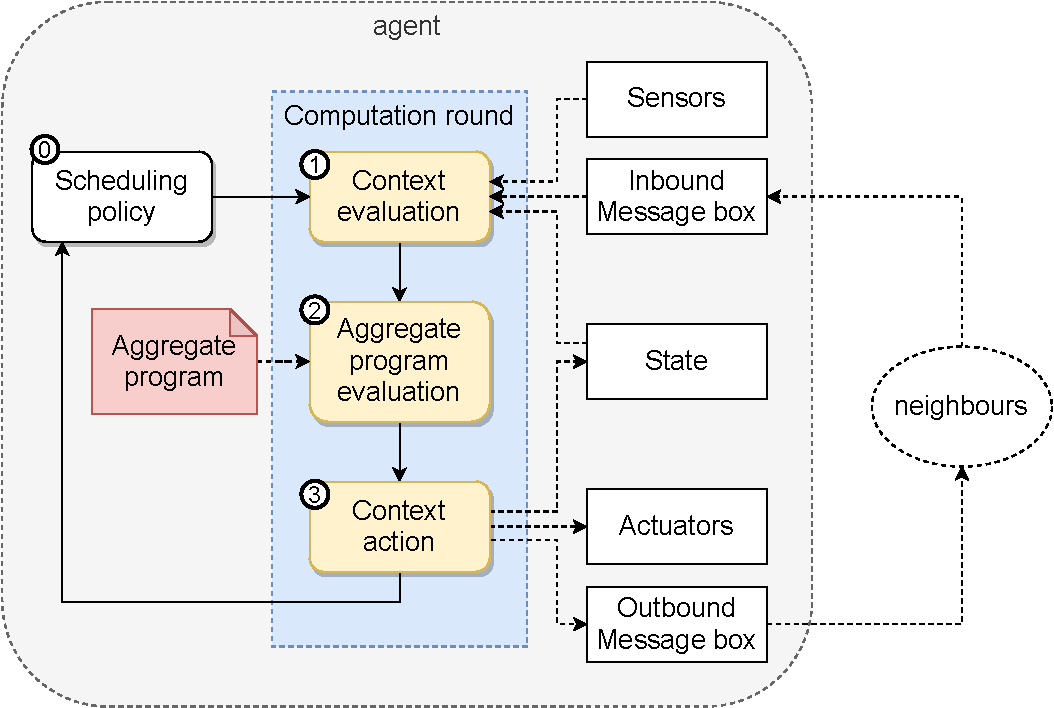
\includegraphics[width=0.8\textwidth]{chapters/img/aggregate-agent-control-architecture.pdf}
    \caption{High level behaviour of an agent in an aggregate system}\label{fig:aggregate-agent-control-architecture}
\end{figure}
%
As per the above consideration,
 the behaviour of any individual agent is best understood
 in terms of repeated action of \emph{execution rounds} (see \Cref{fig:aggregate-agent-control-architecture}), where each round consists of the following steps (though some flexibility exists especially in the actuation part):
%
\begin{enumerate}
\item \emph{Context acquisition.} The agent gathers its context by considering its previous state as well as the most recent sensor readings and messages from neighbours.
\item \emph{Computation.} The agent runs a computation against the acquired context, 
 yielding (i) an \emph{output} describing potential actuations; 
 and (ii) a \emph{coordination message} containing all the information to be sent to neighbours for the purpose of coordination at a collective level.
\item \emph{Actuation \rev{and communication}.} The agent performs the actuations described by the program output and dispatches the coordination message to the entire neighbourhood.
\end{enumerate}
%
\rev{
By having every agent repeatedly
 run these sense-compute-act rounds,
 the whole system
 fosters a self-organization process
 whereby
 up-to-date information
 (from the environment and from the agents)
 is continuously incorporated
 and processed,
 typically in a self-stabilising manner~\cite{DBLP:books/mit/Dolev2000}.
}

This system model provides a basic machinery for collective adaptive behaviour,
 which however requires a proper description of the ``local computation step'': this is fostered by the \emph{field-based programming model} (discussed in \Cref{sec:field-based-programming-model}).
%
\rev{
A \emph{field-based program}
 steers the collective adaptive behaviour of a system,
 which unfolds by having each agent in the system
 evaluate that program
 according to the discussed round-based execution model.
%
Notice that such a program
 specifies both what local processing the agents
 must perform
 and what data they must share with neighbours;
 also, notice that generally, 
 the program does not affect the round-based execution protocol---unless advanced forms of scheduling are desired~\cite{DBLP:journals/lmcs/PianiniCVMZ21,aguzzi2022addressing}.
The distributed execution protocol may be provided by a \emph{middleware},
 which will ensure that
 messages are exchanged
 and rounds properly scheduled.
%
The reader can refer to
 \cite{DBLP:journals/lmcs/PianiniCVMZ21}
 and
 \cite{casadei2022applsci}, respectively,
for a more comprehensive discussion on
 execution and deployment aspects.
}

\subsection{Field-based Programming Model}
\begin{figure}
\begin{align*}
    \boxed{
    \begin{aligned}
    \q{P} &::= \q{F}\ \q{e} && \text{program} \\
    \q{F} &::= \q{def} \, \q{f(}\bar{\q{x}}\q{)} \{\q{e}\} && \text{function declaration} \\
    \q{e} &::= \q{x} \ | \ \q{v} \ | \ \q{f(}\bar{\q{e}}\q{)} \ | \ \q{if}(\q{e})\{\q{e}\}\{\q{e}\} \ | \ \q{nbr}\{\q{e}\} \ | \ \q{rep}(\q{e})\{(\q{x}) \rightarrow \q{e}\} && \text{expression} \\
    \q{f} &::= \q{d} \ | \ \q{b} && \text{function name} \\
    \q{v} &::= \q{l} \ | \ \phi && \text{value} \\
    \q{l} &::= \q{c(}\bar{\q{l}}\q{)} && \text{local value} \\
    \phi &::= \bar{\delta} \mapsto \bar{\q{l}} && \text{neighbouring field value}
    \end{aligned}
    }
\end{align*}
\caption{Field Calculus abstract syntax extracted from~\cite{DBLP:journals/tomacs/ViroliABDP18}.}
\label{fig:field-calculus-abstract-syntax}
\end{figure}
\label{sec:field-based-programming-model}
Field Calculus (FC) was originally conceptualized in~\cite{viroli2013calculus}
 as a foundational framework aimed at capturing essential elements in computational field languages. 
 These elements include field function definitions, 
 functional interplay with fields, 
 time-based field changes, 
 the building of field values from surrounding nodes, 
 and limiting computations to network sub-regions.

One of the distinctive aspects of field calculus is its dual interpretive nature. 
 On a local scale, the specification describes cyclic computations on individual devices 
 (i.e., the system model described above). 
% 
Conversely, at the global level, 
 a field calculus expression maps each computational round for every device to its corresponding space-time value. 
 This inherent duality effectively bridges the gap between individual device behaviour and the emergent global network behaviour,
 a claim supported by computational adequacy and abstraction properties as outlined in~\cite{audrito2019tocl}.

\Cref{fig:field-calculus-abstract-syntax} describes the abstract syntax for field calculus. 
 In this syntax, an overbar notation ($\bar{\q{e}}$) indicates a sequence of elements, 
 namely $\bar{\q{e}}$ stands for $\q{e}_1, \q{e}_2, \ldots, \q{e}_n$ for some $n \geq 0$.
 When multiple overbar notations are used in the same expression,
 they are assumed to have the same length and they are expanded together,
 namely $\bar{\delta} \mapsto \bar{\q{l}}$ stands for $\delta_1 \mapsto \q{l}_1, \delta_2 \mapsto \q{l}_2, \ldots, \delta_n \mapsto \q{l}_n$ for some $n \geq 0$.
 Keywords in this syntax include \texttt{def} for function definitions, 
 \texttt{if} for conditional expressions, 
 and \texttt{rep} and \texttt{nbr} for specific field calculus operations related to time-based state evolution and neighbour data sharing, respectively.

A typical field calculus program $\q{P}$ comprises a series of function declarations $\bar{\q{F}}$ followed by a main expression $\q{e}$, 
 which collectively describes both global and local system behaviour. 
An expression $\q{e}$ can be:
\begin{itemize}
    \item a \emph{variable} $\q{x}$,
    \item a \emph{value} $\q{v}$, which can be either:
    \begin{itemize}
        \item a \emph{local value} $\q{l}$, defined through a constructor $\q{c}$ applied to a sequence of arguments $\bar{\q{l}}$, such as boolean, number, string, etc.
        \item a \emph{neighbouring field value} $\phi$, defined through a sequence of pairs $\bar{\delta} \mapsto \bar{\q{l}}$, where $\bar{\delta}$ is a sequence of neighbouring device (including itself) and $\bar{\q{l}}$ is a sequence of local values, e.g., a map of neighbouring devices to the distance from them.
    \end{itemize}
    \item a function application $\q{f(}\bar{\q{e}}\q{)}$, where $\q{f}$ is a function name and $\bar{\q{e}}$ is a sequence of expressions, e.g., $\q{f(}\q{x}, \q{v}\q{)}$. 
    It can be \emph{user defined}, e.g., $\q{d(}\q{x}\q{)}$, or \emph{built-in}, e.g., $\q{b(}\q{v}\q{)}$.
    \item a \emph{branching expression} $\q{if}(\q{e})\{\q{e}\}\{\q{e}\}$, where $\q{e}$ is a boolean expression and $\q{e}$ is an expression, e.g., $\q{if}(\q{b(}\q{v}\q{)})\{\q{d(}\q{x}\q{)}\}\{\q{v}\}$. 
    \item a \emph{neighbourhood expression} $\q{nbr}\{\q{e}\}$, which creates a neighbouring value mapping neighbours to their latest available result of evaluating e. In particular, each
    device $\delta$:
    \begin{itemize}
        \item shares its value of \texttt{e} with its neighbours, and
        \item evaluates the expression into a neighbouring value $\Phi$, where $\Phi$ is a function that maps each neighbour $\delta'$ of $\delta$ to the latest evaluation of \texttt{e} that
        has been shared from $\delta$
    \end{itemize}
    \item A \emph{neighbourhood expression}, denoted as $\q{nbr}\{\q{e}\}$, 
     generates a mapping that associates neighbours with their most recent evaluation results of \texttt{e}. 
     Specifically, for each device $\delta$:
    \begin{itemize}
        \item It disseminates its evaluation of \texttt{e} to its neighbours.
        \item It computes the expression into a neighbourhood value function $\Phi$. This function $\Phi$ maps each neighbouring device $\delta'$ to the most recent evaluation of \texttt{e} received from $\delta$.
    \end{itemize}
    For example, $\texttt{nbr}(\texttt{humidity()}$) (where \texttt{humidity()} is a built-in sensor estimating local humidity) would result in a neighbourhood value function $\Phi$, 
    which maps each neighbour to the humidity level measured by that neighbour. 
    It is worth noting that in an \texttt{if} statement, 
    sharing is confined to devices within the same branch's subspace.
    This is because devices in different subspaces do not execute the same $\texttt{nbr}(\texttt{e})$ constructs.
    \item $\q{rep}(\q{e})\{(\q{x}) \rightarrow \q{e}\}$, where $\q{e}$ is an expression, $\q{x}$ is a variable, and $\q{e}$ is an expression. 
    It simulates the dynamic evolution of the state over time intervals. 
    This construct extracts the previously computed value \( v \) from the complete \texttt{rep} expression during the last evaluation cycle. 
    For the initial evaluation, the expression \( \texttt{e1} \) is evaluated to provide the starting value of \( v \). In subsequent rounds, 
    \( v \) is updated based on the outcome of evaluating \( \texttt{e2} \),
    where each instance of \( x \) is substituted with \( v \).

\end{itemize}
Within this suite of operations, 
 the \texttt{nbr} and \texttt{rep} constructs serve distinct roles, 
 facilitating message exchanges between devices and managing state within the iterative rounds of an individual device, respectively. 
%
These constructs are underpinned by a data gathering mechanism enabled through a technique known as \emph{alignment}~\cite{audrito2016run}. 
This ensures accurate message correspondence, 
 eliminating the possibility of unintended message swapping between different instances of \texttt{nbr} expressions, 
 as well as preventing state memory interchange between different instances of \texttt{rep} expressions. 
% 
A significant implication of this is the isolated execution of the two branches in a \texttt{if} statement within field calculus; a
  device executing the \texttt{then} branch is unable to communicate with the \texttt{else} branch of a neighbouring device, and vice versa.
%
\subsubsection{Examples}
\label{sec:field-calculus-foundational-behaviour}
The proposed model and language are quite simple and intuitive, 
 yet it is expressive enough to capture a wide range of collective behaviours.
In the following, we present a few examples of collective behaviours that can be expressed in this model.
\paragraph*{Direct neighbour interaction (space)}
In the realm of aggregate computing, 
 one can effectively calculate spatial structures by utilizing the \texttt{nbr} construct. 
 Consider, for example, the task of computing the average temperature perceived by a device along with its neighbouring devices. 
 This can be seamlessly implemented through the \texttt{nbr} construct as shown below:
\begin{lstlisting}[language=scafi]
val totalTemperature = foldhood(0.0)(_ + )(nbr{temperature()})
val neighboursCount = foldhood(0)( + _)(nbr{1})
val averageTemperature = totalTemperature / neighboursCount
\end{lstlisting}
Here, \texttt{foldhood} is a built-in function designed for the aggregation of neighbour values. 
It takes three parameters:
\begin{enumerate}
\item The neutral element, which serves as the initial value for the aggregation.
\item The aggregation function, which defines how the values should be combined.
\item The query to neighbours, which specifies what information is to be collected from each neighbour.
\end{enumerate} 
\paragraph*{Local field evolution (time)}
If with \texttt{nbr} we can collect information from the neighbourhood, 
 with \texttt{rep} we can evolve the state of the device over time. 
 For instance, consider the following example:
\begin{lstlisting}[language=scafi]
rep(0) { local => local + 1}
\end{lstlisting}
This expression initializes the state of the device to 0 and then increments it by 1 in each subsequent round, namely it simulates a counter.
Combining these two operators, it is possible to create space-time patterns, 
 such as the following, that simulates a wave propagating in space.
 One such pattern is the self-healing gradient.
\paragraph*{Self-healing gradient (space-time)}
A gradient is a field that associates each device in the system with its shortest distance to the nearest source device. 
 A \emph{self-healing} gradient algorithm calculates this gradient field and autonomously 
 updates it to reflect alterations in the source set or network connectivity. 
 This algorithm is significant because it frequently serves as a component in more complex self-organizing algorithms, 
 such as those used for managing information flows, gathering distributed data, and segmenting networks into regions.
 Using the field calculus, this can be expressed as follows:
\begin{lstlisting}[language=scafi]
// distance from source region with nbrRange metric
def distanceTo(source) {
    rep (Infinity) { 
        (dist) =>
            mux (source) { 0 } 
            { minHood(nbr{dist} + nbrRange()) }
    }
}
\end{lstlisting}
where \lstinline|mux| is a conditional expression, 
 \lstinline|minHood| is a built-in function that returns the minimum value in the neighbourhood, 
 and \lstinline|nbrRange| is a built-in function that returns neighbouring field distance.

 \subsubsection{Aggregate programming stack}
Building upon both theoretical insights and pragmatic considerations, 
 aggregate programming introduces a stratified architecture designed to significantly ease the design, development, and maintenance of intricate distributed systems. 
 This methodology stems from three pivotal observations related to engineering sophisticated coordination schemas:
\begin{itemize}
    \item the composition of modules and subsystems should be straightforward and transparent.
    \item various subsystems necessitate distinct coordination mechanisms that are context-sensitive, varying according to regions and temporal conditions.
    \item robust coordination mechanisms should be encapsulated within abstractions, thereby obviating the need for programmers to grapple with their underlying complexities.
\end{itemize}
Field calculus, along with its language incarnations, 
 offers solutions for the first two observations but falls short of ensuring resilience. 
 Additionally, its mathematical rigour and concise syntax present challenges for straightforward programming. 
 Consequently, supplementary methodologies are indispensable for scaling effectively with system complexity.
 These pattern have been identified in literate~\cite{aggregatecomputing} and are called resilient coordination operators (more details in \Cref{sec:field-calculus-building-blocks} and \Cref{sec:field-calculus-behavioural-properties}).
 Finally, on top of these operators, there are high-level patterns that can be used to implement complex behaviours (more details in \Cref{sec:field-calculus-high-level-patterns}) and high-level API for structuring domain-specific behaviour (e.g., crowd detection or coordinate movement in swarms).
 The overall stack is shown in \Cref{fig:aggregate-programming-stack}.
\begin{figure}
    \centering
    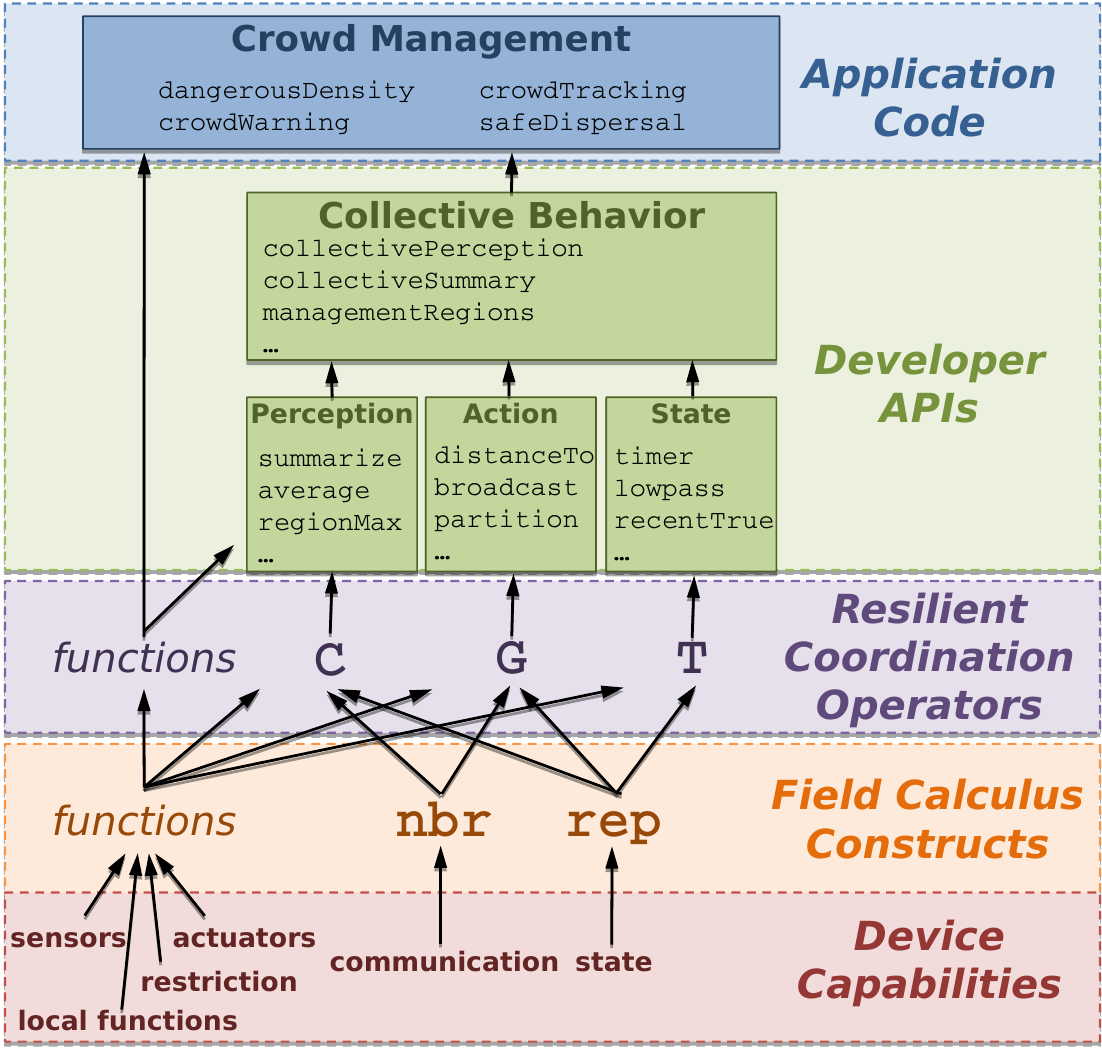
\includegraphics[width=0.5\textwidth]{chapters/img/aggregate-programming-stack.png}
    \caption{The aggregate programming stack}\label{fig:aggregate-programming-stack}
\end{figure}
\subsubsection{Resilient coordination operators}
\label{sec:field-calculus-building-blocks}
Throughout the development of aggregate computing, 
 a consistent set of foundational building blocks has emerged over the years. 
 These building blocks are known for their self-stabilizing properties--
 details on which will be discussed later--
 and they serve as the foundation for various high-level patterns in aggregate computing.
\paragraph*{Gradient-cast (G)}
Various forms of aggregation 
 can be executed along a distance gradient.
 Essentially, a generalized operator G serves as a gradient algorithm. 
 This algorithm is tailored based on a specific \emph{metric} used for measuring increments or distances. 
 It enables the transfer of a particular field value from the source in an outward direction, 
 evolving according to a specified logic as it ascends the gradient.
\paragraph*{Collect-cast (C)}
In essence, G facilitates the flow of information from originating devices to their broader environment, 
 acting as a mechanism for the spread or diffusion of values. 
 Conversely, a secondary operation enables data to flow from a widespread area to specific gathering points, 
 aiding in decentralized sensing tasks. 
 This is enabled by another generalized operator, C shown in Figure 7.13b. C accumulates values along a potential field, beginning at source points where the potential is highest, and aggregates these values as it moves down the parent chain, eventually converging at points where the potential is lowest.
\paragraph*{Sparse choice (S)}
The generic operator Sparse choice (S) 
 allows for the selective inclusion of devices to divide the network into distinct ``responsibility zones''. Essentially, it performs a leader election procedure. 
 In this process, a ``grain'' represents the average distance between two elected leaders, as defined by a specific metric. It can be implemented as follows:

\subsubsection{Behavioural Properties}\label{sec:field-calculus-behavioural-properties}
The field calculus is architected as a universal language specifically tailored for computations in spatially distributed systems. 
 One of the most critical properties studied within subsets of this core language is that of \emph{self-stabilization}, 
 which ensures the system's ability to autonomously reach a correct state~\cite{lafuente2015fixpoint}%~\cite{Dol00, LLM17, LLM15}.
 Defined formally within the context of the transition system \( N \stackrel{\text{act}}{\rightarrow} N \) representing network evolution, self-stabilization guarantees that:
\begin{enumerate}
    \item the program evaluation, given an eventually constant input, 
    will converge to a stable value at each device within a finite timeframe.
    \item This stable value is solely determined by the current input values, 
    thus mitigating any interference from transitory states.
\end{enumerate}

Self-stabilizing algorithms are particularly robust in dynamically evolving systems, 
 reacting coherently to input changes without residual influence from prior states.

The study in~\cite{damiani2015type}
 identifies an initial set of self-stabilizing fragments through a `spreading operator', 
 which performs monotonic updates on neighbouring values through a diffusion function. 
 These fragments allow for versatile combinations with local operations, 
 excluding explicit \texttt{rep} and \texttt{nbr} expressions. 
 Nevertheless, this framework supports several fundamental building blocks like distance estimation and broadcast.

An expanded set of self-stabilizing fragments and building blocks are covered in~\cite{viroli2018engineering}. 
 This work proposes usage restrictions on \texttt{rep} statements to specific patterns: 
 \emph{converging}, \emph{acyclic}, and \emph{minimising}. 
 These correlate with the three primary building blocks: 
 G, C, and T, each with distinct functionalities and applications. 
 Moreover, the study delves into the notion of `equivalence and substitutability' for self-stabilizing programs. 
 This concept not only allows for program optimization through the substitution of more efficient equivalents but also provides a new lens for understanding self-stabilizing programs by abstracting their transient behaviours.

The work establishes different semantic interpretations of a given program: 
 operational semantics (local viewpoint), denotational semantics (global viewpoint), and eventual behaviour (limit viewpoint). 
 Another perspective, termed as the `continuous viewpoint,' is explored in~\cite{beal2017self}. 
 This involves the convergence of output values towards a continuous function, 
 as the density of computing devices in an area increases.

Taking cues from self-stabilization principles, 
 the notion is relaxed to define `eventually consistent' programs. 
 These programs are expected to converge to a limit continuously, 
 barring a transient initial period, assuming that the inputs remain constant beyond this initial period. This eventual consistency is demonstrated for all programs expressible in the GPI calculus~\cite{audrito2018space}.

Lastly, 
 contemporary work is beginning to examine the real-time performance guarantees of field calculus programs~\cite{audrito2018space}. 
 Current validation approaches primarily focus on `by construction' proofs based on elementary building blocks or restricted fragments of the calculus. 
\subsubsection{High-level patterns}\label{sec:field-calculus-high-level-patterns}
Starting from the previous defined building blocks, 
 it is possible to define high-level patterns that can be used to implement complex behaviours.
 One of the most promising approaches is the one based on the \emph{self-organising coordination regions} (SCR) pattern~\cite{casadei2019scr}.
\paragraph*{Self-Organising Coordination Regions (SCR)}
In a more advanced scenario, 
 one could employ the SCR design pattern. 
 The core objective of the SCR pattern is to partition a decentralized system into distinct spatial zones, each overseen by a designated leader device. 
 This leadership device is responsible for consolidating data from other devices within its jurisdiction,
 and subsequently disseminating decisions that enforce policies across the entire region.

For example, 
 in a large-scale project aimed at monitoring and controlling temperature, 
 the SCR pattern allows the formation of uniformly-sized regions. 
 Within these zones, devices collaboratively compute the area's average temperature. 
 Using this aggregated information, the system could trigger alarms, facilitating more effective, coarse-grained analysis and intervention measures.
%
This pattern is implemented using the G, C and S operators as follows:

\subsection{Tools}
Proper software tooling
is essential to new self-organising algorithms
and variants or extensions of the aggregate programming model,
promoting scientific and technological progress.
In the following, we present ScaFi--a Scala-based aggregate programming framework--and Alchemist--a meta-simulator for aggregate computing.
\subsubsection{ScaFi}\label{sec:scafi}
%!TeX root = thesis-main.tex
 \emph{\scafi{} (Scala-Fields)} is
 an aggregate programming toolkit
 that comprises an internal DSL (language and virtual machine)
 as well as supporting components for the simulation
 and execution %deployment 
 of aggregate systems.

\subparagraph{Software description}
\label{}
\scafi{} is a multi-module Scala project hosted on GitHub\footnote{\url{https://github.com/scafi/scafi}}.
%
It provides DSL and API modules for 
 writing, testing, and running aggregate programs, namely programs expressed according to the aggregate programming paradigm~\cite{aggregatecomputing,DBLP:journals/jlap/ViroliBDACP19}.
%
\subparagraph{Software Architecture}
\label{sec:scafi-arch-design}

The high-level architecture of \scafi{} is depicted in \Cref{fig:scafi-arch}.
It consists of the following main components: %(where each component is an SBT module and deployable artifact):
\begin{itemize}
\item \texttt{scafi-commons} | provides basic abstractions and utilities (e.g., spatial and temporal abstractions);
\item \texttt{scafi-core} | provides an aggregate programming DSL (syntax, semantics, and a virtual machine for evaluation of programs), together with a ``standard library'' of reusable functions;
\item \texttt{scafi-stdlib-ext} | provides extra library functionality that requires external dependencies and is hence kept separated from the minimalist \texttt{scafi-core};
\item \texttt{scafi-simulator}: provides basic support for simulating aggregate systems;
\item \texttt{scafi-simulator-gui} | provides a GUI for visualizing and interacting with simulations of aggregate systems;
\item \texttt{spala} (``spatial Scala''---i.e., a general aggregate computing platform\footnote{aggregate computing is rooted in spatial computing~\cite{DBLP:journals/corr/abs-1202-5509}.}) | provides an actor-based aggregate computing middleware
(independent of the \scafi{} DSL and potentially applicable to other aggregate programming languages as well)
based on the Akka toolkit~\cite{akka};
\item \texttt{scafi-distributed} | ScaFi integration-layer for \texttt{spala},
which can be leveraged to set up actor-based deployments of \scafi{}-programmed systems.
\end{itemize}
 
\begin{figure}
\centering
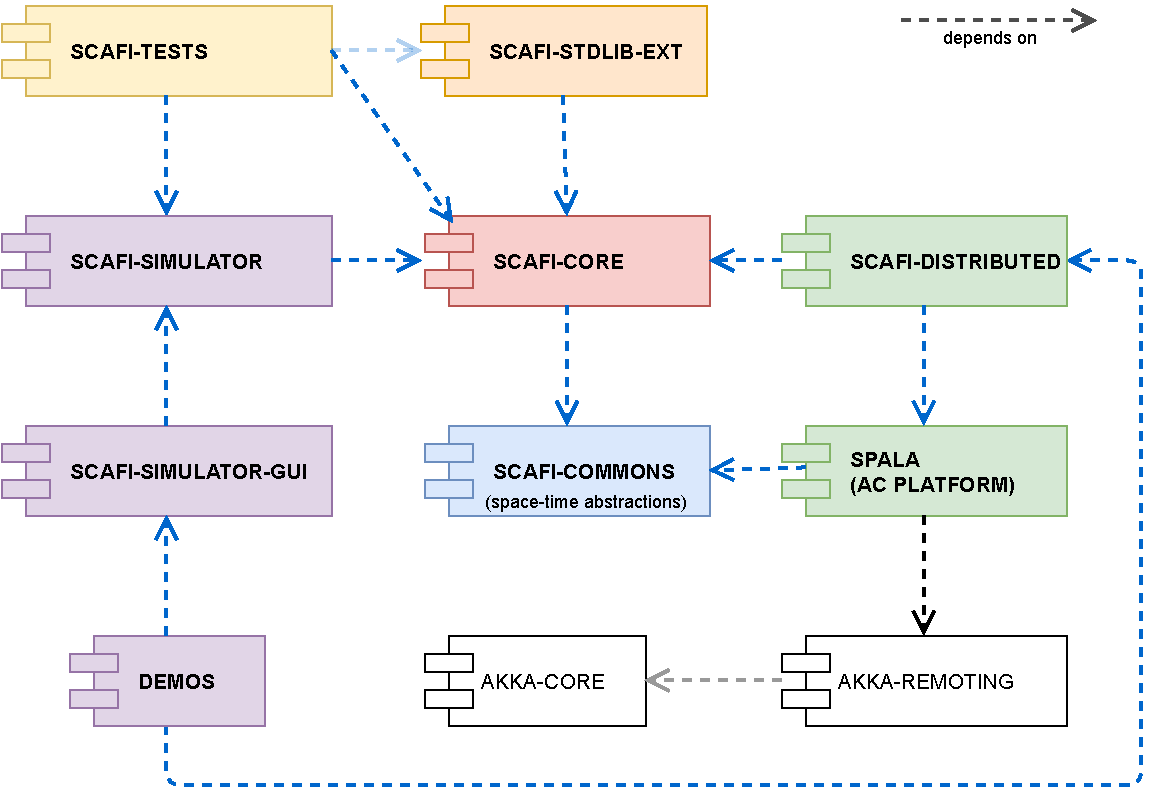
\includegraphics[width=0.8\textwidth]{papers/softwarex2021/imgs/scafi-project-org.pdf}
\caption{High-level architecture of the \scafi{} toolkit.}
\label{fig:scafi-arch}
\end{figure}

\begin{figure}
\centering
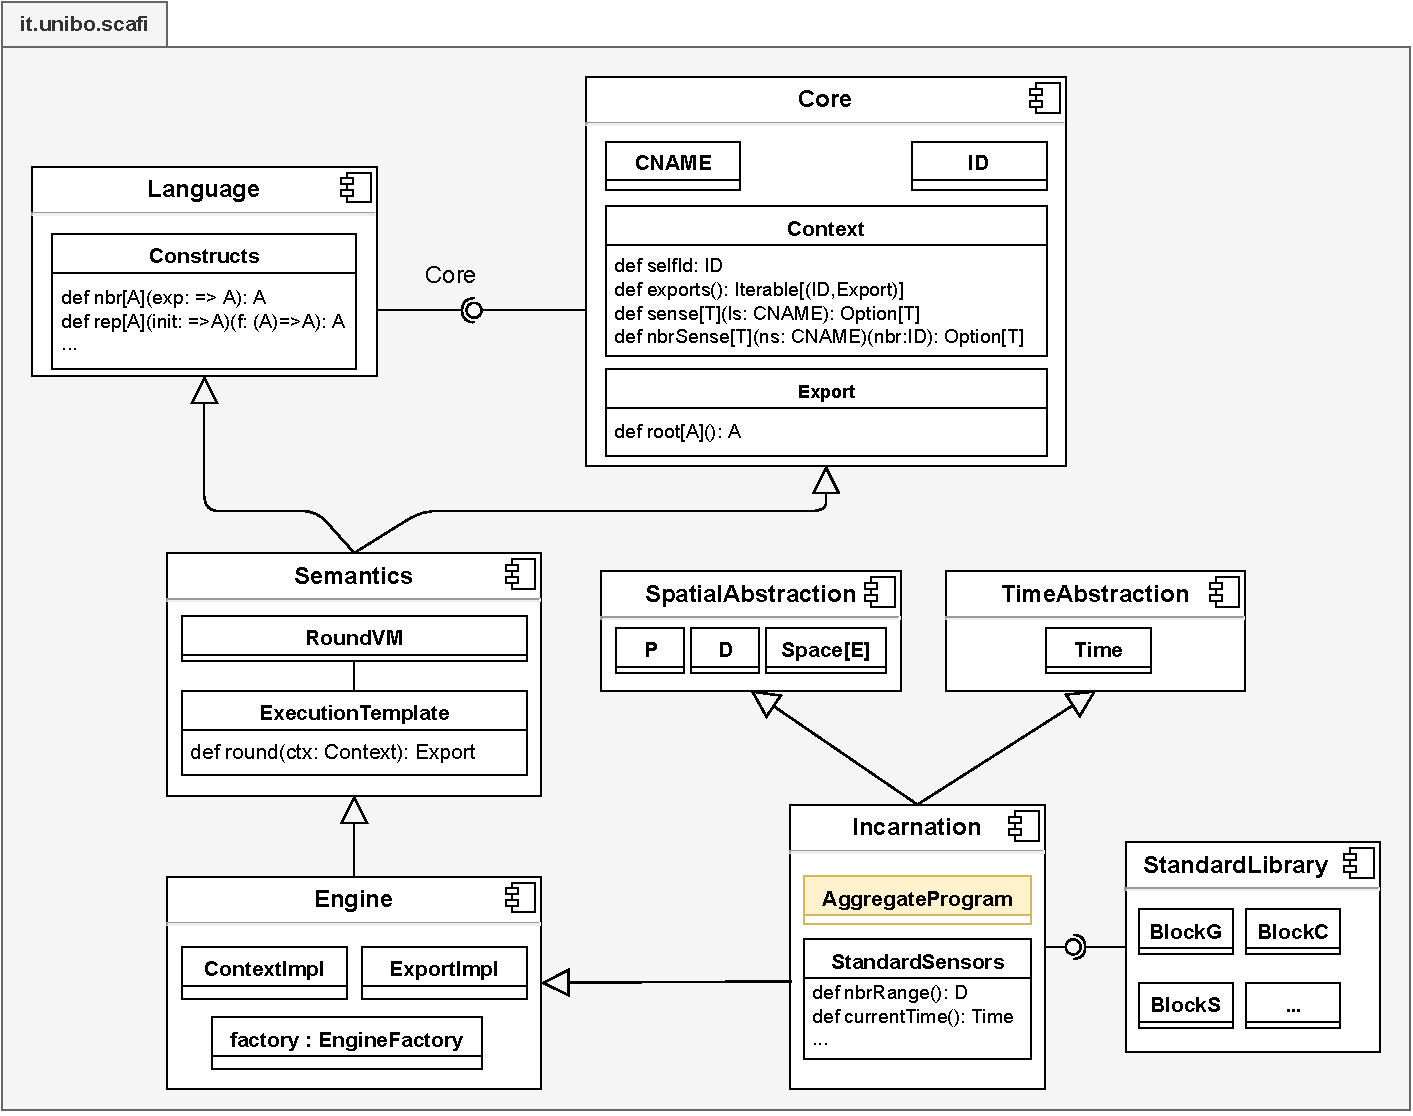
\includegraphics[width=0.8\textwidth]{papers/softwarex2021/imgs/scafi-design.drawio.pdf}
\caption{\revision{Design of the core of \scafi{} (DSL).}}
\label{fig:scafi-design}
\end{figure}

\revision{
\scafi{} leverages the concept of an \emph{incarnation},
 namely a concrete ``family of types''~\cite{DBLP:conf/oopsla/OderskyZ05} 
 that is progressively refined through inheritance, composed, and finally instantiated into an object (cf. the Scala \emph{cake pattern}~\cite{Hunt2013cakepattern,DBLP:conf/oopsla/OderskyZ05})
 which ultimately provides access 
 to a type-coherent set of features.

\Cref{fig:scafi-design} provides an excerpt 
 of the main Scala traits 
 with some types and objects they define.
%
Trait \texttt{Core} provides the abstract fundamental types: \texttt{CNAME} for capability names,
\texttt{ID} for device identifiers,
\texttt{Context} for the input environment of computation rounds,
and \texttt{Export} for the outcomes of computation rounds.
%
Trait \texttt{Language} 
 provides the syntax of the DSL in terms of methods, through interface \texttt{Constructs}.
%
Trait \texttt{Semantics} and \texttt{Engine}
 implement the DSL construct semantics,
 providing a template for \texttt{AggregateProgram} base class defined in the \texttt{Incarnation} trait. 
The incarnation also exposes \texttt{StandardSensors} in terms of, e.g., \texttt{SpatialAbstraction}'s and \texttt{TimeAbstraction}'s types for positions (\texttt{P}), distances (\texttt{P}), and time.
%
The \texttt{StandardLibrary} is provided by leveraging 
 what an incarnation provides,
 providing traits of functionality to be mixed into \texttt{AggregateProgram}s.
}

\paragraph*{Software Functionalities}
\label{}

\subparagraph*{Expressing aggregate programs through a Scala DSL}
\label{sec:express-programs}
%
Module \texttt{scafi-core}
 exposes,
 through incarnations,
 an \texttt{AggregateProgram} trait
  that provides access to 
  aggregate programming constructs---following 
  a variant of the field calculus~\cite{DBLP:journals/tocl/AudritoVDPB19,DBLP:journals/jlap/ViroliBDACP19}
  formalized in~\cite{DBLP:conf/isola/CasadeiVAD20}.
%
This single program defines -- from a global perspective -- 
 the collective adaptive behaviour 
 of an entire %system or 
 ensemble of computational devices.
%
Besides the core constructs,
 this module also provides ``standard library'' traits
 providing access to reusable functions of aggregate functionality.
%
For instance, by mixing trait \texttt{Gradients}
 into an \texttt{AggregateProgram} subclass,
 a developer gets access to \emph{gradient functions}~\revision{\cite{DBLP:conf/sac/BealBVT08,DBLP:journals/tomacs/ViroliABDP18}}, used to 
 continuously compute (over space and time) the self-healing field of minimum distances of each node from a set of source nodes. %---possibly in mobile and faulty environments.
%
Several such traits are available
 to provide other key building blocks
 for self-organising applications~\revision{\cite{DBLP:conf/saso/WolfH07,DBLP:journals/tomacs/ViroliABDP18}} (e.g., \texttt{BlockG} \revision{for gradient-wise information propagation}, \texttt{BlockC} \revision{for gradient-wise information collection}, \texttt{BlockS} \revision{for sparse choice or leader election})
 or experimental language features
 (e.g., the \texttt{spawn} function for concurrent aggregate processes~\revision{\cite{DBLP:journals/eaai/CasadeiVAPD21,testa2022processes}}\revision{, for modelling independent and overlapping aggregate computations}).
%
\subparagraph*{Virtual machine for the local execution of aggregate programs}
%
An \texttt{AggregateProgram} instance 
 is a function
 mapping a \texttt{Context}
 (the set of inputs needed by an individual device
  to properly evaluate the program locally)
 to an \texttt{Export}
 (the tree of values that has to be shared 
  with neighbours to effectively coordinate and promote 
  the emergence of collective behaviours).
%
Using this API,
 a developer can 
 integrate ``aggregate functionality''
 into its system---what remains to be specified are the
 details of the aggregate execution model and the communication among devices,
 that may change in different applications.
%
Devices must continuously run the aggregate program,
but the scheduling of these computation rounds can be tuned
as the application needs~\cite{DBLP:journals/lmcs/PianiniCVMZ21}.
%
\texttt{Export}s must be shared with neighbouring devices to allow them
to properly set up their \texttt{Context}s,
but the network protocol to be used to do so can be selected
independently of the program.
 
\subparagraph*{Simulation support}
%
In order to simulate an ``aggregate system'',
 it is necessary to: 
\begin{enumerate}
  \item define the set of computational devices that make up the aggregate, including their sensors and actuators;
  \item define the aggregate topology, i.e., 
  some application-specific \emph{neighbouring relationship}
  from which the set of \emph{neighbours}
  of each device can be determined;
  \item define the aggregate program to be executed;
  \item define a certain dynamics of the system
  by proper scheduling of computation rounds,
  and the environment
  by proper scheduling of changes in sensor values.
\end{enumerate}

%
Module \texttt{scafi-simulator}
 provides this basic support.
%
It exposes some factory methods
to configure simulations properly
 (e.g., it supports ad-hoc and spatial distance-based connectivity rules)
 and an API to run and interact with simulations.
%
Then, module \texttt{scafi-simulator-gui}
 provides a convenient graphical user interface
 to launch and visually show simulations in execution.
%
We remark that these modules currently support basic simulation scenarios
 and are mainly meant for quick experiments
 or as a starting basis for ad-hoc simulation frameworks.
 
\subparagraph*{Experimental or work-in-progress features: actor-based middleware}
%
Regarding the construction of actual systems, 
 \scafi{}
 provides
 an actor-based implementation
 of the aggregate execution model~\cite{DBLP:series/lncs/CasadeiV18},
 in the \texttt{spala} (\texttt{Spa}tial Sca\texttt{la}) module,
 which is instrumental for integrating aggregate computing
 into existing systems and distributed architectures~\cite{DBLP:series/lncs/CasadeiV18}.
%
Indeed, aggregate computing systems
 can be designed, deployed, and executed 
 according to different
 architectural styles 
 and concrete architectures~\cite{DBLP:journals/fi/CasadeiPPVW20}.
%
So, \scafi{} provides \emph{two} main implementations of the middleware,
 in package \texttt{it.unibo.scafi.distrib.actor},
 for purely peer-to-peer 
 (sub-package \texttt{p2p})
 and server-based designs
 (sub-package \texttt{server}).
%
The main abstraction
 is the \texttt{DeviceActor},
 which exposes a message-based interface
 for controlling and interacting with
 an individual logical node of the aggregate system.
%
Then, an object-oriented façade API is provided to set up a system of middleware-level actors. 

%\subparagraph{Sample code snippets analysis (optional)}
%\label{}

%\subparagraph{Illustrative Examples}
\paragraph*{Features}
\label{s:impact}
\scafi{}
 has been used 
 in aggregate computing-related research~\cite{DBLP:journals/eaai/CasadeiVAPD21,audrito2022ecoop-xc,DBLP:conf/coordination/AguzziCV22,
 DBLP:conf/fmec/CasadeiV19,DBLP:conf/IEEEscc/CasadeiTVD19,DBLP:journals/scp/CasadeiAV18,DBLP:journals/jsan/CasadeiAV21,DBLP:conf/coordination/CasadeiVRA21,casadei2022applsci,arxiv2020scafi-nc},
  touching themes such as 
  software engineering, 
  computational models, and
  distributed systems/algorithms.
%
The impact of \scafi{}
 can be understood in terms of 
 existing and prospective contributions, 
 discussed in the following.

\subparagraph*{Interplay between programming language design and foundational research} 
%
The implementation of the \scafi{} DSL
 has inspired a variant of the field calculus
 which arguably supports easier embeddability
 into mainstream programming languages~\cite{DBLP:conf/isola/CasadeiVAD20,arxiv2020scafi-nc}.

\subparagraph*{High-level programming models}
%
The previous discussion  
 makes the case for ``DSL stacking''~\cite{DBLP:conf/icsoft/HummE10}.
%
Indeed, by leveraging the aforementioned aggregate process extension, 
 it is possible to reduce the abstraction gap
 needed to implement \emph{situated tuples}~\cite{DBLP:conf/coordination/CasadeiVRA21}\revision{,
 which is a Linda-like model~\cite{DBLP:journals/toplas/Gelernter85} for coordinating processes where tuples and tuple operations are situated in space}.
%
By mapping high-level specifications into aggregate programs, it is sometimes straightforward to develop resilient distributed implementations---as in~\cite{DBLP:journals/jss/AudritoCDSV21},
 where translation rules from 
 spatial logic formulas
 to field calculus expressions
 enable seamless construction of decentralized monitors for such formulas.

\subparagraph*{Web-friendliness}
%
By leveraging Scala.js~\cite{DBLP:conf/scala/Doeraene18}, \scafi{} can be easily 
 accessed through JavaScript,
 which promotes cross-platform language design 
 and reuse of functionality in the browser
 (to support web applications without the need of server-side components).
%
This paved the path 
 to \scafiweb{}~\cite{DBLP:conf/coordination/AguzziCMPV21},
 a web playground for aggregate programming.
%

\subsubsection{Alchemist}\label{coordination2023:alchemist}
Alchemist\footnote{\url{http://alchemistsimulator.github.io/}}~\cite{alchemist} is meta-simulator
 mainly designed for simulating complex distributed systems 
 in a rich variety of scenarios like swarm robotics~\cite{aguzzi2023macroswarm},
 large-scale sensor networks~\cite{Aguzzi_2022}, crowd simulation~\cite{aggregatecomputing},
 path planning, and even morphogenesis of multi-cellular systems.

The simulator is \emph{meta} in nature, 
 as it is based on general abstractions 
 that can be mapped to specific use cases (i.e., \emph{incarnations}).
% 
Inspired by biochemistry, 
 the meta-model consists of a set of \emph{nodes} 
 that exist in an \emph{environment} and are linked together by \emph{relationship} rules. 
 Each node contains a sequence of \emph{molecules} and \emph{reactions}. 
%
 A \emph{molecule} represents a variable, 
 which acts as a container for data. 
 \emph{Reactions} instead are events that occur based 
 on a set of \emph{conditions}, 
 and are fired according to a time distribution, 
 producing an effect that is described as an action. 
This abstraction allows the simulator to be flexible 
 and adaptable to a variety of use cases and node numbers 
 (it could support thousands of nodes), 
 while maintaining a consistent underlying structure.

 The Alchemist simulator features four incarnations: 
  biochemistry, Sapere, Protelis, and \scafi{},
  each with a different way of modelling molecules and actions.
The latter is the reference of this thesis since it supports the \scafi{} Scala DSL
 the current reference framework for aggregate computing in Scala.

Alchemist offers an effortless method for loading simulations. 
 The process requires a YAML file that includes essential parameters, 
 such as the incarnation type, neighbour connection model, and node deployment. 
 In \Cref{coordination2023:fig:alchemist}, we have provided an example YAML file 
 that creates a simulation using the \scafi{} incarnation (first row). 
 It also defines the neighbourhood relationship based on fixed distances (0.5 in this case), 
 placing nodes in a fixed grid of size 10x10 starting at -(5,5) and ending at (5,5), 
 with a node-to-node distance of 0.25. 
 Finally, it loads the \scafi{} program called ``program'', 
 which is evaluated at each node with a frequency of 1. 
\begin{figure*}
\centering
\begin{subfigure}[b]{0.49\textwidth}
    \centering
    %% change the listing size to small with the correct font family
    \begin{lstlisting}[language=yaml, basicstyle=\small\ttfamily, caption={An Alchemist simulation example.}, captionpos=b, label=coordination2023:fig:alchemist-yaml]
incarnation: scafi
network-model:
    type: ConnectWithinDistance
    parameters: [0.5]
deployments:
    type: Grid
    parameters: [-5,-5,5,5,0.25,0.25]
    /*dynamics of the simulation*/
    programs: 
        - program:
        - time-distribution: 1
            type: Event
            actions: 
            - type: RunScafiProgram
              parameters: [program]
        - program: send
\end{lstlisting}
\end{subfigure}
\hfill
\begin{subfigure}[b]{0.49\textwidth}
    \centering
    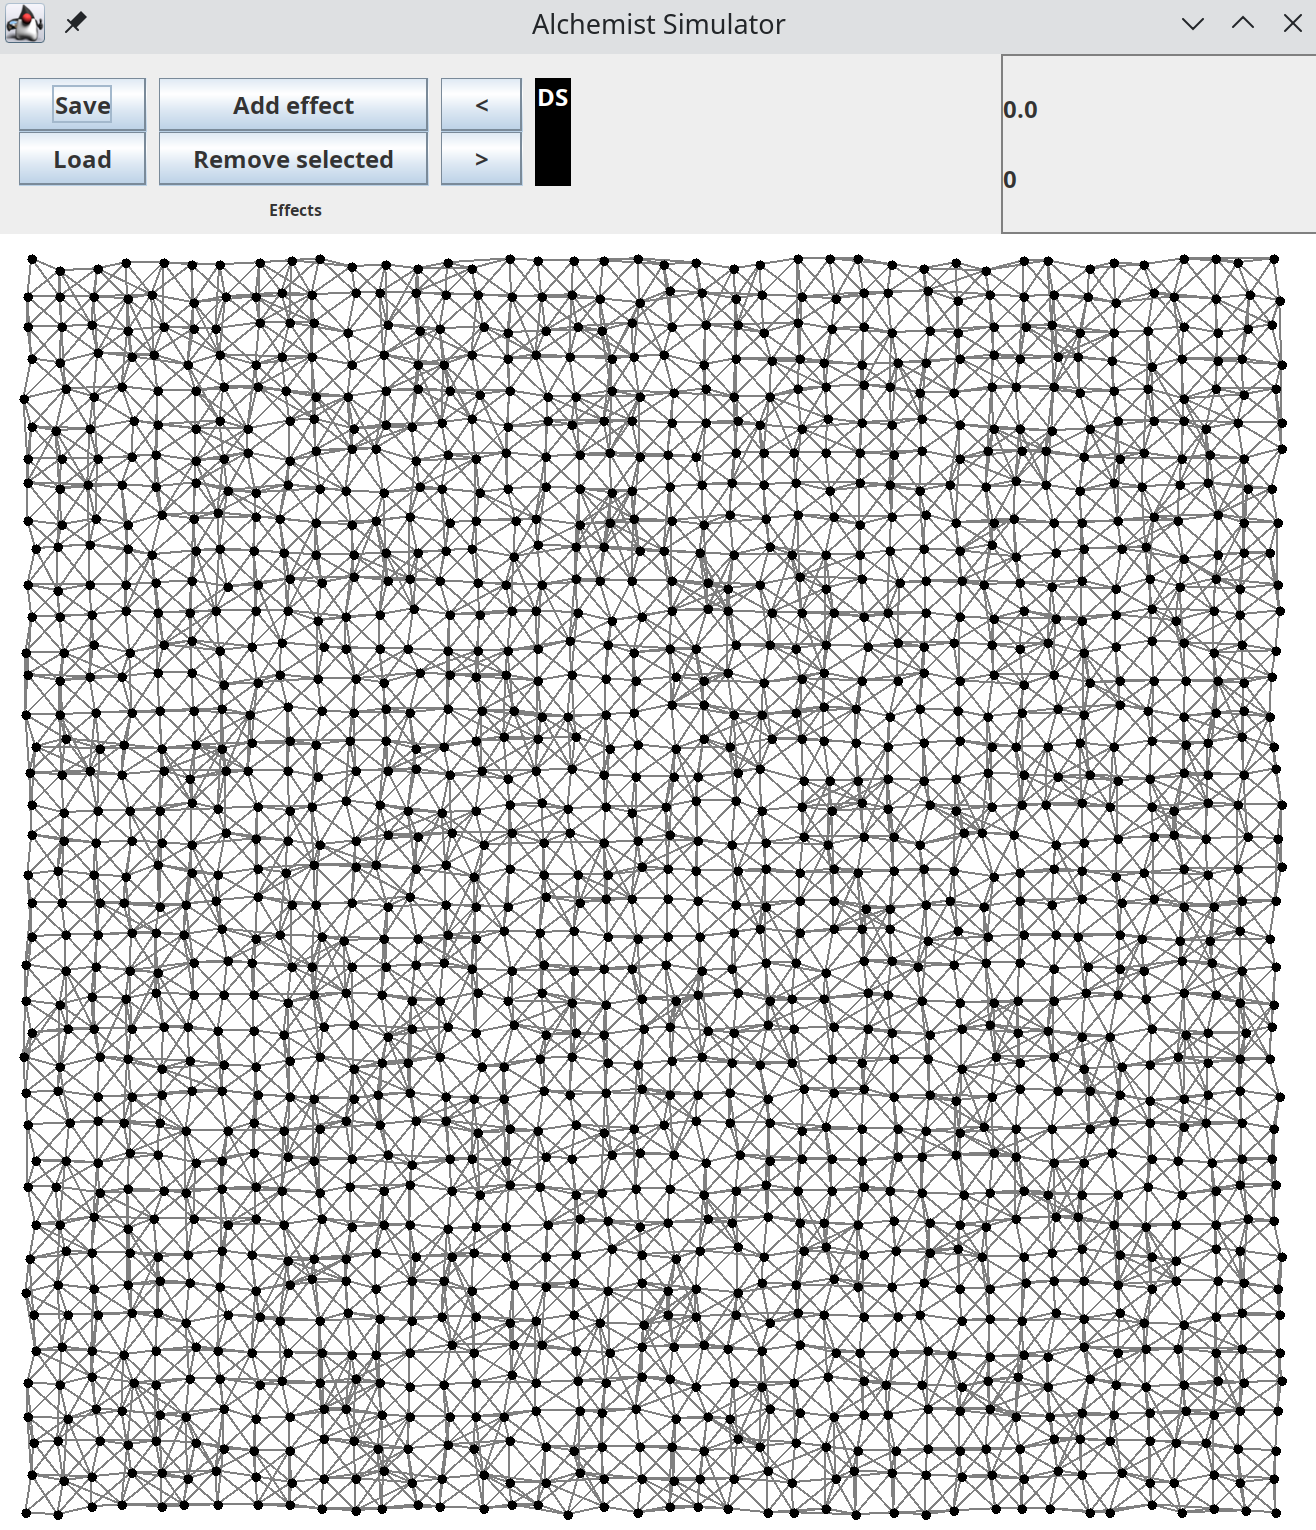
\includegraphics[width=\textwidth]{papers/coordination2023/imgs/alchemist.png}
\end{subfigure}
\caption[An Alchemist simulation example]{An Alchemist simulation example. 
    The simulation result on the right is obtained 
    by running the simulation described on the left.
    }
\label{coordination2023:fig:alchemist}
\end{figure*}

\section{Final Remarks}
Addressing collective adaptive behaviour is a long-standing research challenge in the realm of complex systems. 
 Macro programming has emerged as a promising approach to bridge the abstraction gap between the problem space and the solution space. 

In this chapter, 
 we provide an overview of the key concepts within this programming paradigm and introduce aggregate computing---a specialized macro programming technique for orchestrating collective self-organizing behaviours in highly scalable and distributed systems. 
 While this paradigm has already found applications in the field of \ac{cpsw}, 
 we identify several areas for further improvement:
\begin{itemize}
    \item A high-level interface tailored for effectively programming behaviours specific to the \ac{cpsw} domain, such as movement, pattern formation, and collective decision-making.
    \item Appropriate abstractions to facilitate the design and development of intricate \ac{cpsw} systems.
    \item Innovative algorithms to enable complex collective behaviours, like sensing-driven clustering.
    \item Robust deployment strategies that accommodate modern, complex IT architectures.
    \item The incorporation of machine learning techniques to overcome current limitations in the state-of-the-art foundational frameworks.
\end{itemize}

%\printbibliography